\documentclass[12pt]{article}
\usepackage[a4paper, margin=2cm]{geometry}
\usepackage[english]{babel} % To obtain English text with the blindtext package
\usepackage{blindtext}
\usepackage{graphicx} % Required for inserting images
\usepackage{array, multirow} % For extra column formatting
\usepackage{amsmath, amssymb, cancel} %for equation environment
\usepackage{float}
\usepackage{parskip} % For gaps between para
\usepackage{setspace}
\usepackage{pdfpages}
\usepackage{abstract}
\usepackage[export]{adjustbox}
\usepackage{emptypage}
\usepackage{tocloft}
\usepackage[nottoc]{tocbibind}
\usepackage{hyperref, url}
\usepackage[table, dvipsnames]{xcolor}
\usepackage{minted}
    \usemintedstyle{monokai}
\usepackage{caption}
    \captionsetup{font=footnotesize,labelfont=bf}
\usepackage{tcolorbox}
    \newtcolorbox{mintedbox}{
        colback=backcolour,
        boxrule=0pt,
        sharp corners,
        width=\linewidth,
        left=0pt, right=0pt,
        top=3pt, bottom=3pt
    }

\cftsetindents{section}{0em}{2em}
\cftsetindents{subsection}{0em}{2em}

\renewcommand\cfttoctitlefont{\hfill\Large\bfseries}
\renewcommand\cftaftertoctitle{\hfill\mbox{}}

\graphicspath{ {./images/} }

\pagenumbering{arabic}

\definecolor{blurple}{HTML}{5865F2}
\definecolor{backcolour}{HTML}{272823}

\hypersetup{
    colorlinks=true,
    linkcolor=black,
    urlcolor=blurple,
    citecolor=blurple,
}

\urlstyle{same}

\renewcommand{\arraystretch}{1.3}

\setcounter{secnumdepth}{5}
\setcounter{tocdepth}{5}
\newcommand\simpleparagraph[1]{%
  \stepcounter{paragraph}\paragraph*{\theparagraph\quad{}#1}}

%%%%%%%%%%%%%%%%%%%%%%%%%%%%%%%%%%%


\title{PHYC20080 Exp.3 Wheatstone}
\author{Joana Adao}
\date{\today}

\begin{document}

\begin{titlepage}
    \begin{center}

        \begin{figure}[ht]
            
\includegraphics[width=\textwidth]{UCDLogo.png}
        \end{figure}
        
        \begin{figure}
            \centerline{
\includegraphics[width=\paperwidth]{UCDBanner.png}}
        \end{figure}

        \vspace{4cm}

        {\LARGE \bfseries PHYC20080 Fields, Waves and Light}\\
        \vspace{0.75cm}
        {\Large Experiment No.3 Determination of the Resistivity of a Metal Alloy Using a Wheatstone Bridge}
        
        \vspace{1cm}
    
    {\Large \textbf{4 March 2025}}
    
    \vspace{2cm}
    
    {\large \textbf{by Joana C.C. Adao (Student No. 23311051)}}\\
    \vspace{.25cm}
    {\large With Beau Etac}\\
    \vspace{0.25cm}
    {\large Tuesday 16.00-18.00 Slot}\\
    {\large Nicki (Coordinator)}

    \end{center}
    
   \clearpage

\end{titlepage}

\setcounter{page}{1}
\tableofcontents

\newpage

\begin{abstract}
\addcontentsline{toc}{section}{Abstract}

The aim of this experiment was to determine the resistance of a metal alloy wire using a Wheatstone bridge setup. By balancing the current across this bridge
and measuring the lengths associated with the resistors (at the point of balance), the resistance ratio formula was applied to find the unknown resistance of the metal alloy wire
to be $\mathbf{1.99 \; \pm \; 0.14 \; \Omega}$. With the found dimensions for the cross-sectional area, the resistivity of the metal alloy wire was then found to be
$\mathbf{8.26 \times 10^{-7} \; \pm \; 1.24 \times 10^{-7} \; \Omega m}$. While this result was determined to be closest to the resistivity expected from stainless steel, constantan
was considered to be the more likely material of the wire due to its common use in electrical circuits. Errors in determining the resistivity likely arose from experimental errors when finding
the unknown resistance of the wire. By ensuring the connections on the Wheatstone brdige were properly secured and by doing additional measurements of resistance accuracy on the values could be improved.

\end{abstract}

%%%%%%%%%%%%%%%%%%%%%%%%%%%%%%%%%%%

\vspace{4cm}

\section{Theory} \label{sec:1}

\subsection{Resistance}

\textbf{Resistance (R)} is a force that opposes the flow of current in a circuit
\cite{flukeresistance,hiokiresistance,britresistance}.
It can be described as the difficulty the electric charge faces when travelling through a medium.
\cite{hiokiresistance}
There are two types of materials that have opposing resistances \cite{flukeresistance}:
\begin{itemize}
    \item \textbf{Conductors:} materials with little resistance where electrons travel through easily; for example copper and gold (as well as most metals).
    \item \textbf{Insulators:} materials where electrical charge finds difficulty passing through; for example wood and rubber.
\end{itemize}
These properties can be seen in electrical wires, with the current-carrying copper wire encased in an insulating rubber tube for safety.

Resistors are circuit components specifically made to counteract the flow of current in a circuit
\cite{britresistor,bbcresistance,hiokiresistance} (Figure \ref{fig:resistor}).
They can be used in an electrical circuit to control the amount of voltage and current flowing in it, which is used to ensure the circuit doesn't blow and to also 
correctly distribute the current/voltage flowing through the circuit
\cite{britresistor,hiokiresistance}
The surplus of electrical energy flowing through a resistor is converted into heat energy which then dissipates
\cite{hiokiresistance}.

\begin{figure}[H]
    \centering
    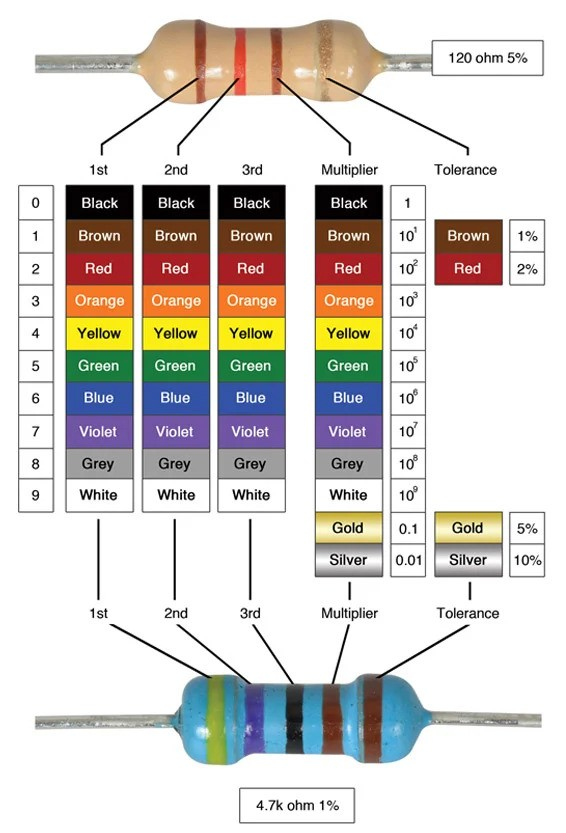
\includegraphics[width=7cm]{resistorr.jpg}
    \caption{\centering Image of resistor and guide on how to read it \protect\cite{resistorpic}}
    \label{fig:resistor}
\end{figure}

Resistors are used everywhere in day-to-day life as it is a basic circuit component. The most notable usages are for laptop (see figure \ref{fig:laptop}) and phone chargers (see figure \ref{fig:phone}),
which often have tens of resistors controlling the flow of the current to each different component of the laptop. Chargers often have the amount of current that
specific charger allows the flow of, which is determined by the amount and type of resistor used \cite{resistorapp}.

\vspace{1ex}
\begin{minipage}{.45\textwidth}
    \captionsetup{hypcap=false}
    \centering
    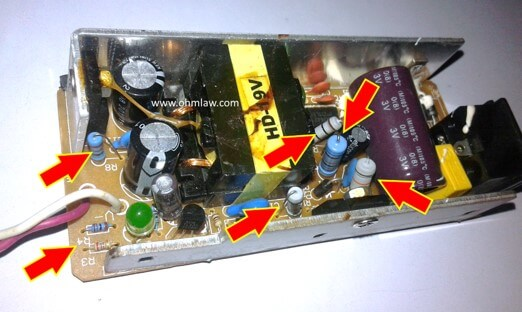
\includegraphics[width=\linewidth]{laptop-charger.jpg}
    \captionof{figure}{\centering Image of a laptop charger with resistor(s) highlighted \protect\cite{resistorapp}.}
    \label{fig:laptop}
\end{minipage}
\hfill
\begin{minipage}{.45\textwidth}
    \captionsetup{hypcap=false}
    \centering
    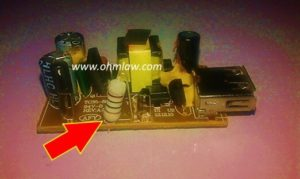
\includegraphics[width=\linewidth]{mobile-phone-charger.jpg}
    \captionof{figure}{\centering Image of a phone charger with resistor(s) highlighted \protect\cite{resistorapp}.}
    \label{fig:phone}
\end{minipage}

\textbf{Resistivity} ($\mathbf{\rho}$) is a property of a material that describes how much that material opposes the flow of current through it. It is a property that
is usually dependent on temperature or pressure rather than its physical factors (ie. shape, size, etc.).

The resistance depends on resistivity of a material, as well as length (L) and cross-sectional area (A). The equation for this relation is given below,

\vspace{-2ex}
\begin{gather} \label{eq:0}
    R = \frac{\rho L}{A}
\end{gather}

As is seen, $R \propto L$, therefore if the length doubles the resistance will also double. In a similar but opposite fashion, $R \propto \dfrac{1}{A}$, therefore if the
\textbf{radius} of the cross-sectional area doubles then the resistance will decrease proportionally by a factor of 4 as area is defined as $A = \pi r^2$.

\subsection{Wheatstone Bridge}

The Wheatstone bridge is a basic electrical circuit consisting of a power source, a \textbf{galvanometer} (G) (a highly sensitive ammeter), 3 resistors of
known resistance and 1 resistor of unknown resistance ($R_x$) (see figure \ref{fig:diagwheat}, \ref{fig:instruwheat}). A Wheatstone bridge is just an instrument used
to measure the resistance of the unknown resistor to high precision when it is compared to other resistors of known resistances \cite{allenwheat, librewheat}.

\vspace{1ex}
\begin{minipage}{.35\textwidth}
    \captionsetup{hypcap=false}
    \centering
    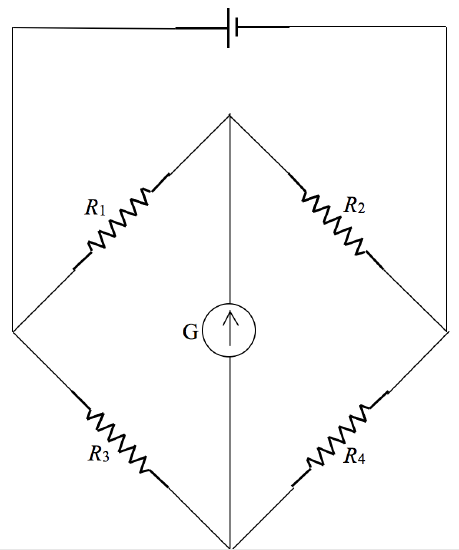
\includegraphics[width=\linewidth]{wheatstone bridge diagram.png}
    \captionof{figure}{\centering Diagram of a Wheatstone bridge setup \protect\cite{librewheat}.}
    \label{fig:diagwheat}
\end{minipage}
\hfill
\begin{minipage}{.55\textwidth}
    \captionsetup{hypcap=false}
    \centering
    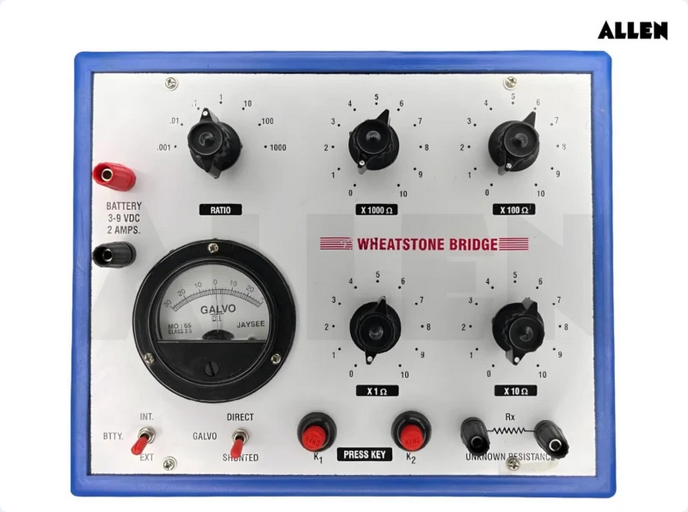
\includegraphics[width=\linewidth]{wheatstone bridge instrument.png}
    \captionof{figure}{\centering Image of typical Wheatstone bridge instrument \protect\cite{allenwheat}.}
    \label{fig:instruwheat}
\end{minipage}

\subsubsection{Derivation of the Wheatstone Bridge Resistor Relation}

First, the wheastone bridge circuit is easier to understand when it is simplified and labelled (see figure \ref{fig:simplewheat}):

\begin{figure}[H]
    \centering
    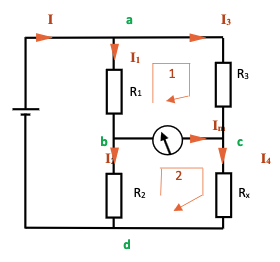
\includegraphics[width=7.5cm]{simplified wheat diagram.png}
    \caption{\centering Simplified and labelled Wheatstone bridge diagram \protect\cite{PHYC20090ass1sol}}
    \label{fig:simplewheat}
\end{figure}

With the simplified circuit it is clear to see that the relation is consisted of series and parallel combinations. By application of Kirchoff's laws at each
junction, the following is found (as junctions \textbf{\textcolor{Green}{a}} and \textbf{\textcolor{Green}{d}} consider just I):

\vspace{-2ex}
\begin{gather} \label{eq:1}
    \text{At junction \textbf{\textcolor{Green}{b}},} \qquad\quad I_1 = I_2 + I_m
\end{gather}
\vspace{-5ex}
\begin{gather} \label{eq:2}
    \text{At junction \textbf{\textcolor{Green}{c}},} \qquad\quad I_4 = I_3 + I_m
\end{gather}

With $I_m$ as the current through the galvanometer and $I_x$ ($x=1,2,3,4$) the current through each resistor. 
At loop 1 (involving resistors $R_1$ and $R_3$) and at loop 2 (involving resistors $R_2$ and $R_x$) the following can be understood:

\vspace{-2ex}
\begin{gather} \label{eq:3}
    \text{At loop 1,} \qquad\quad V_{R_1} - V_{R_3} + V_m = 0 \: \implies \: I_1R_1 - I_3R_3 + I_mR_m = 0
\end{gather}
\vspace{-5ex}
\begin{gather} \label{eq:4}
    \text{At loop 2,} \qquad\quad V_{R_2} - V_m - V_{R_x} = 0 \: \implies \: I_2R_2 - I_mR_m - I_4R_x = 0
\end{gather}

The positive/negative values taken for each component are dependent on wether the current flows in the same/opposite direction to the specificied loop respectively.
But the unknown resistance can only be found when the bridge is balanced, therefore $I_m = 0$,

\vspace{-2ex}
\begin{align*}
    (1) \quad \implies \quad I_1 = I_2 \\
    (2) \quad \implies \quad I_4 = I_3
\end{align*}

As is expected with resistors in series. And the following can also then be said when $I_m=0$,

\vspace{-2ex}
\begin{align*}
    (3) \quad \implies \quad I_1R_1 = I_3R_3 \\
    (4) \quad \implies \quad I_2R_2 = I_4R_x
\end{align*}

But the new relationship for (\ref{eq:1}) and (\ref{eq:2}) can be used in (\ref{eq:3}) to find:

\vspace{-2ex}
\begin{gather} \label{eq:5}
    I_2R_1 = I_4R_3
\end{gather}

(\ref{eq:5}) can then be divided by (\ref{eq:4}) to get rid of the currents and thus the relationship between resistors in a \textit{balanced} Wheatstone bridge is found:

\vspace{-2ex}
\begin{gather} \label{eq:6}
    \frac{R_1}{R_2} = \frac{R_3}{R_x}
\end{gather}

(\ref{eq:6}) can be manipulated to solve for the unknown resistance, $R_x$:

\vspace{-2ex}
\begin{gather} \label{eq:7}
    R_x = R_3 \; \frac{R_2}{R_1}
\end{gather}

\section{Methodology} \label{sec:2}

The apparatus was connected as shown in figure \ref{fig:setup}, with a metal alloy wire of unknown resistance connected to one of the bridges.
For the simplicity of this experimental setup, the resistor relation in a wheatstone bridge can make use of the fact that $R \propto L$ to infer from (\ref{eq:6}),

\vspace{-2ex}
\begin{gather} \label{eq:9}
    \frac{R_1}{R_x} = \frac{L_1}{L_2}
\end{gather}

The ratio difference between lengths associated with the respective resistors ($R_1 \propto L_1$, $R_x \propto L_2$) allows for the calculation of the unkown resistance.

\begin{figure}[H]
    \centering
    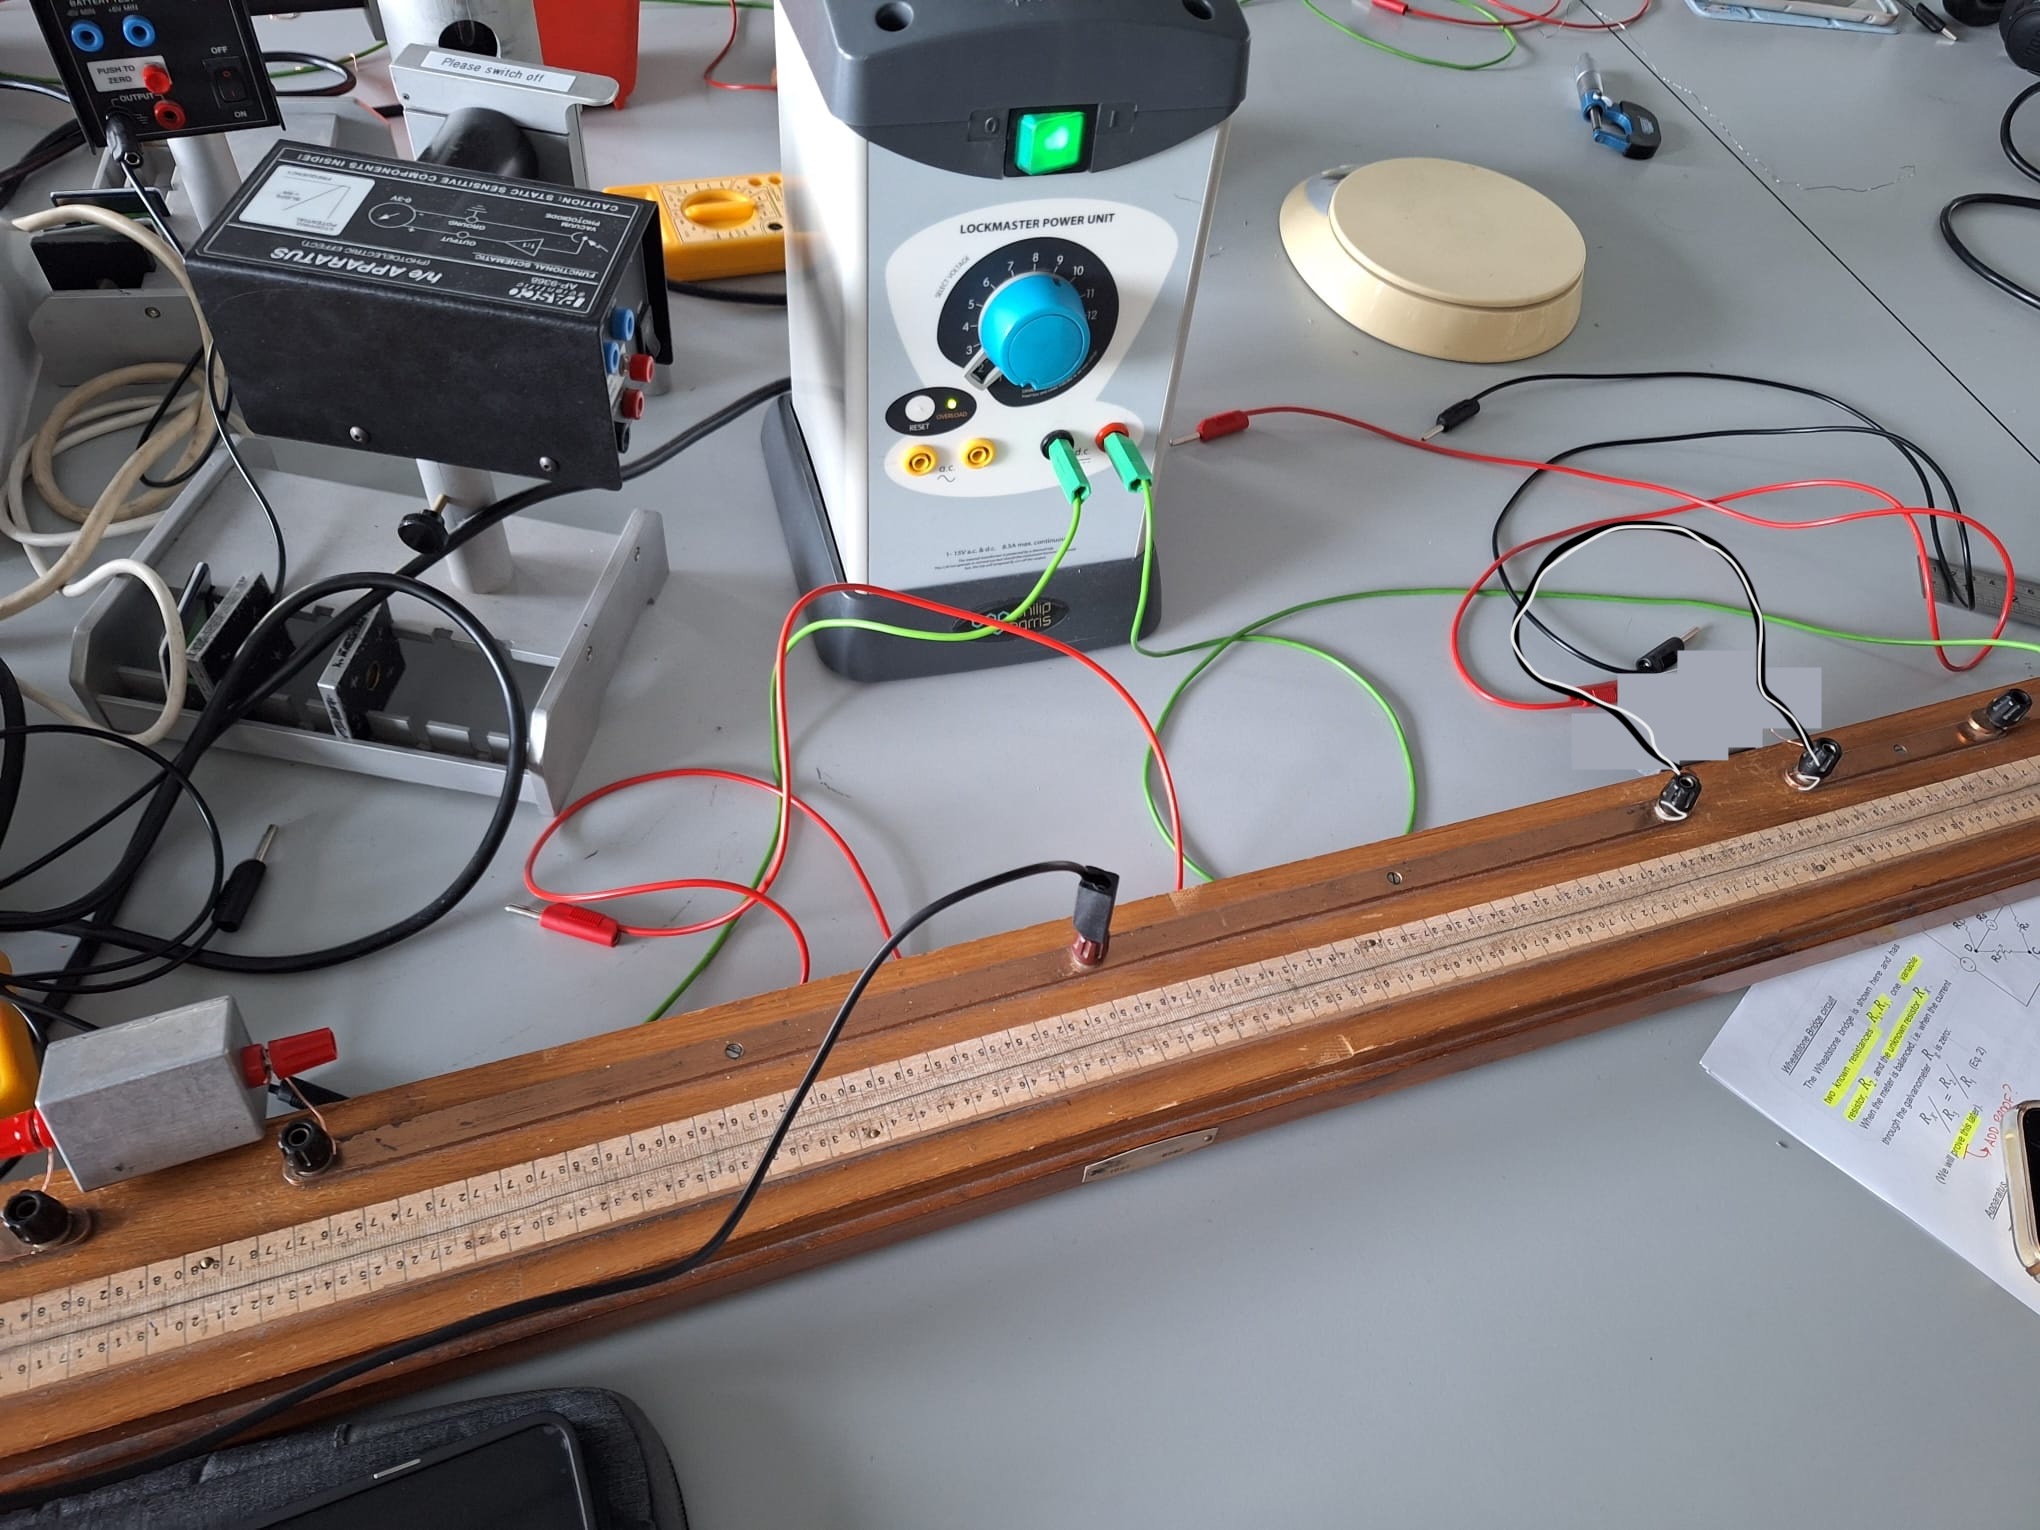
\includegraphics[width=.75\textwidth]{wheatstone apparatus.jpeg}
    \caption{\centering Image of the apparatus setup with wire alloy of unknown resistance drawn in.}
    \label{fig:setup}
\end{figure}

The respective lengths of each resistor is measured from the point when the contact maker (manual galvanometer) is stable at 0 (no deflections, balanced). These measurements are
recorded including the resistance of the known resistor.

The known resistance resistor and metal alloy wire of unknown resistance swap places in order to verify equipment is functioning. If results differ by more than 1 cm, it is likely that the 
meter bridge has poor contacts. This can be fixed by tightening the contacts at every point.

The average value for the unknown resistance is then found and the associated uncertainty by calculating the standard deviation.

The resistivity of the metal alloy wire can be found by using a micrometer to measure the average diameter of the wire (average of 6 measurements taken at different places) and using that value
to find the average cross-sectional area. This calculated value can be plugged into equation \ref{eq:0} to then find the resistivity of the wire.

\section{Results and Calculations} \label{sec:3}

The known resitance resistor was chosen, at random, to be $\mathbf{0.97 \Omega}$. After successfully connecting the metal alloy wire to the metre bridge, the system was found to be balanced
at lengths 0.308 m ($L_1$) and 0.692 m ($L_2$). By equation (\ref{eq:9}) the unknown resistance $R_x$ is found to be,

\vspace{-2ex}
\begin{gather*}
    R_x = R_1 \; \frac{L_2}{L_1} \: = \: 0.97 \cdot \frac{0.692}{0.308} \: = \: \mathbf{2.18 \; \Omega}
\end{gather*}

So $R_x$ is found to be $\mathbf{2.18 \Omega}$. When the position of the metal alloy wire and resistor are switched, the legnths at which the bridge is balanced are found to be
0.322 m ($L_1$) and 0.678 m ($L_2$). Though these measurements differ by more than 1 cm the experiment was allowed to proceed with these values. By equation (\ref{eq:9}) again the unkown resistance $R_x$ is now found to be,

\vspace{-2ex}
\begin{gather*}
    R_x = R_1 \; \frac{L_2}{L_1} \: = \: 0.97 \cdot \frac{0.678}{0.322} \: = \: \mathbf{2.04 \; \Omega}
\end{gather*}

So $R_x$ is found to be $\mathbf{2.04 \; \Omega}$.
Taking the average between these two values, the unknown resistance $R_x$ of the metal alloy wire is found to be $\mathbf{2.11 \; \Omega}$.

A similar process was done for the same metal alloy wire but with differing known resistance resistors. The follow table is then compiled with the results found and calculated:

\begin{table}[H]
    \centering
    \caption{Table of the values gathered for length and the calculated respective $R_x$ values.}
    \label{tab:1}
    \begin{tabular}{cccc}
    \hline
    $\mathbf{R_1 \: (\Omega)}$ & $\mathbf{L_1 \: (\text{\textbf{m}})}$ & $\mathbf{L_2 \: (\text{\textbf{m}})}$ & $\mathbf{R_x \: (\Omega)}$ \\ \hline \hline
    \rowcolor[HTML]{EFEFEF} 
    0.97 & 0.308 & 0.692 & 2.18 \\
    \rowcolor[HTML]{EFEFEF} 
    0.97 & 0.322 & 0.678 & 2.04 \\
    0.94 & 0.302 & 0.698 & 2.17 \\
    2.71 & 0.619 & 0.381 & 1.67 \\
    4.74 & 0.659 & 0.341 & 2.45 \\
    1.87 & 0.571 & 0.429 & 1.40 \\ \hline
    \end{tabular}%
\end{table}

The average value of the above unknown resistances $R_x$ is found to then be $\mathbf{1.99 \; \Omega}$. With a standard deviation value of 0.350, the standard error ($SE,R_x$) is found to be:

\vspace{-2ex}
\begin{gather*}
    SE,R_x \: = \: \frac{\sigma}{\sqrt{N}} \: = \: \frac{0.350}{\sqrt{6}} \: = \: \mathbf{0.14 \; \Omega}
\end{gather*}

Therefore, the average resistance for the metal alloy wire $R_x$ is found to be $\mathbf{1.99 \; \pm \; 0.14 \; \Omega}$.

The resistivity of the metal alloy wire can then be found using this value. The average diameter of the wire is found to be 0.49 mm (from 0.45 mm, 0.50 mm, 0.55 mm, 0.45 mm, 0.45 mm, 0.55 mm) and the
length of the wire is found to be 0.455 m. The average cross-sectional area of the wire is then calculated to be:

\vspace{-2ex}
\begin{gather*}
    A \: = \: \pi r^2 \: = \: \pi \left( \frac{0.49 \times 10^{-3}}{2} \right)^2 \: = \: 1.90 \times 10 ^{-7} \; m
\end{gather*}

So the average resistivity of the wire (at room temperature) can then be calculated by equation (\ref{eq:0}),

\vspace{-2ex}
\begin{gather*}
    \rho \: = \: \frac{RA}{L} \: = \: \frac{(1.99)(1.90 \times 10^{-7})}{0.455} \: = \: \mathbf{8.26 \times 10 ^{-7} \; \Omega m}
\end{gather*}

The error on the resistivity can be found using error propagation:

\vspace{-2ex}
\begin{gather*}
    \Delta \rho = \rho\left( \frac{\Delta R}{R} + \frac{\Delta A}{A} + \frac{\Delta L}{L} \right)
\end{gather*}

With this formula, the average resistivity of the metal alloy wire with the associated error is then found to be $\mathbf{8.26 \times 10^{-7} \; \pm \; 1.24 \times 10^{-7} \; \Omega m}$ (\textit{refer to the Appendix for the calculations code}).

\vspace{3.5cm}

\section{Conclusion} \label{sec:4}

By carrying out this experiment the resistance of the metal alloy wire (unknown resistance) was found to be $\mathbf{1.99 \; \pm \; 0.14 \; \Omega}$ and the resistivity of the same
wire was calculated to be $\mathbf{8.26 \times 10^{-7} \; \pm \; 1.24 \times 10^{-7} \; \Omega m}$. By comparing to a table of the found values of resistivities for different metals \cite{resistvity},
the calculated value is closest to the resistivity of stainless steel ($\rho = 6.9 \times 10^{-7} \; \Omega m$), but the most probable material that the metal alloy wire was made of is constantan ($\rho = 4.9 \times 10 ^{-7} \; \Omega m$) (55\% copper, 45\% nickel)
purely due to its common usage in electrical circuits. Neither of these values are within the calculated error of allowance for resistivity, so there were likely issues during the measurement of the resistances for the wire. Errors for those measurements of the
unknown resistances were likely from poor or unstable connections of the Wheatstone bridge. This could be fixed by ensuring all of the connections are firmly secured and tightened.
More measurements for the unknown resistance using more known resistors could have also improved accuracy. 

\newpage

%%%%%%%%%%%%%%%%%%%%%%%%%%%%%%%%%%%

\bibliographystyle{IEEEtran}
\bibliography{References} \label{sec:ref}

\vspace{1.5cm}

\listoffigures

\listoftables

\section*{Appendix} \label{sec:A}
\addcontentsline{toc}{section}{Appendix}

\subsection*{Code}
\addcontentsline{toc}{subsection}{Code}

%

\begin{minipage}{\linewidth}
\captionsetup{hypcap=false}

\begin{mintedbox}
\begin{minted}[fontsize=\small, breaklines, baselinestretch=1.2, xleftmargin=0.5cm]{python}
import numpy as np

L = np.array([0.455, 0.455, 0.455, 0.455, 0.455, 0.455])
dL = np.array([0.0005, 0.0005, 0.0005, 0.0005, 0.0005, 0.0005])

R = np.array([2.18, 2.17, 1.67, 2.45, 1.40, 2.04])
aR = np.average(R)
dR = np.std(R)/np.sqrt(np.size(R))

print(aR, r"$\pm$", dR) # avg R and SE on R

r = (np.array([0.45, 0.45, 0.45, 0.50, 0.55, 0.55]) * 1e-3) /2
ar = np.average(r)

A = np.pi * (r)**2
aA = np.pi * (ar)**2

dA = np.std(A)/np.sqrt(np.size(A))

print(aA, r"$\pm$", dA) # avg A and SE on A

rho = (R*A)/L # for this to work on python had to add the resistance from switched wire position so the arrays were the same size
arho = np.average(rho)
drho = rho * ( (dR/R) + (dA/A) + (dL/L))
adrho = np.average(drho)

print(arho, r"$\pm$", adrho)

\end{minted}
\end{mintedbox}

\captionof{figure}{\centering Code for calculations in §\ref{sec:3}.}
\end{minipage}

\end{document}